\documentclass[12pt]{beamer}
\usepackage[utf8]{inputenc} % style d'écriture
\usepackage[T1]{fontenc}      % package
\usepackage[francais]{babel}  % package pour langue française
\usepackage{graphicx}
\usepackage{subcaption}
\usepackage{url}
\usepackage{color}
\usepackage{geometry}
\usepackage{amssymb}

% William PENSEC, étudiant en Master 2 2020/2021

\usetheme[secheader]{Madrid}
\beamertemplatenavigationsymbolsempty
\setbeamertemplate{frametitle continuation}{}

\title[Compte rendu de stage 1]{Coopération de drones dans un système hétérogène}
\subtitle{Compte rendu de stage 1}
\author{William \textsc{Pensec}}
%\author{William \textsc{Pensec}}
%\author{William \textsc{Pensec}}
\institute{Lab-Sticc}
\date{20/04/2021}

\AtBeginSection[]
{
\begin{frame}<beamer>{Sommaire}
\tableofcontents[currentsection,currentsubsection, 
    hideothersubsections, 
    sectionstyle=show/shaded,
]
\end{frame}
}

\begin{document}
	% ---------------------------------------------------------------- %
	\begin{frame}
		\begin{titlepage}
			\begin{figure}[H]
				\centering
				
\includegraphics[scale=.15]{labsticc.png}
				\hspace{3cm}
				
\includegraphics[scale=.3]{ubo.png}
			\end{figure}
		\end{titlepage}
	\end{frame}
	
	% ---------------------------------------------------------------- %
	\section*{Sommaire}
	\begin{frame}
		\frametitle{Sommaire}
		\begin{center}
			\tableofcontents
		\end{center}
	\end{frame}
	
	% ---------------------------------------------------------------- %
	\section{Sujet}
	\subsection{Contexte}	
	\begin{frame}[allowframebreaks]
	\frametitle{Contexte}
		\begin{exampleblock}{L'industrie du futur}
				\begin{itemize}
					\setbeamertemplate{itemize item}[cercle]
					\item De plus en plus digitalisée et automatisée
					\item Équipements fortement hétérogènes (protocoles réseaux, systèmes employés, quantités d'informations à analyser)
					\item Notion de systèmes cyber-physiques dans le but de tracer les chaînes de production
				\end{itemize}
		\end{exampleblock}
		
		\begin{exampleblock}{Utilisation des drones}
				\begin{itemize}
					\setbeamertemplate{itemize item}[cercle]
					\item Champs d'applications divers $\rightarrow$ surveillance de zone, diagnostic d'infrastructure
					\item Accompagnement du processus de fabrication de manière autonome grâce aux capteurs et caméras disponibles
					\item Capacité de transmissions de données et/ou d'analyse
					\item Nombreuses possibilités d'automatisation
				\end{itemize}
		\end{exampleblock}
	\end{frame}
	
	% ------------------------------- %
	\subsection{Problématique}	
	\begin{frame}
	\frametitle{Problématique}
		\begin{exampleblock}{}
			\begin{itemize}
				\setbeamertemplate{itemize item}[triangle]
				\item Coopération entre le drone et les dispositifs présents dans la chaîne de production
				\item Assurer différentes opérations comme la prise d'image d'une panne, le suivi de la production, surveillance de l'environnement sans risques
			\end{itemize}
		\end{exampleblock}
	\end{frame}
	
	% ------------------------------- %
	\subsection{Fonction}
	\begin{frame}[allowframebreaks]
	\frametitle{Fonction}
		\begin{exampleblock}{}
				\begin{itemize}
					\setbeamertemplate{itemize item}[square]
					\item Découverte de l'environnement opérationnel
					\item Connecter le drone à la partie industrielle
					\item Analyse de données par le drone
				\end{itemize}
		\end{exampleblock}
	\end{frame}
	
	
	
	% ---------------------------------------------------------------- %
	\section{Réalisation}
	\subsection{Prise en main de la plate-forme}
	\begin{frame}
	\frametitle{Plate-forme}
		\begin{figure}[H]
			\centering
			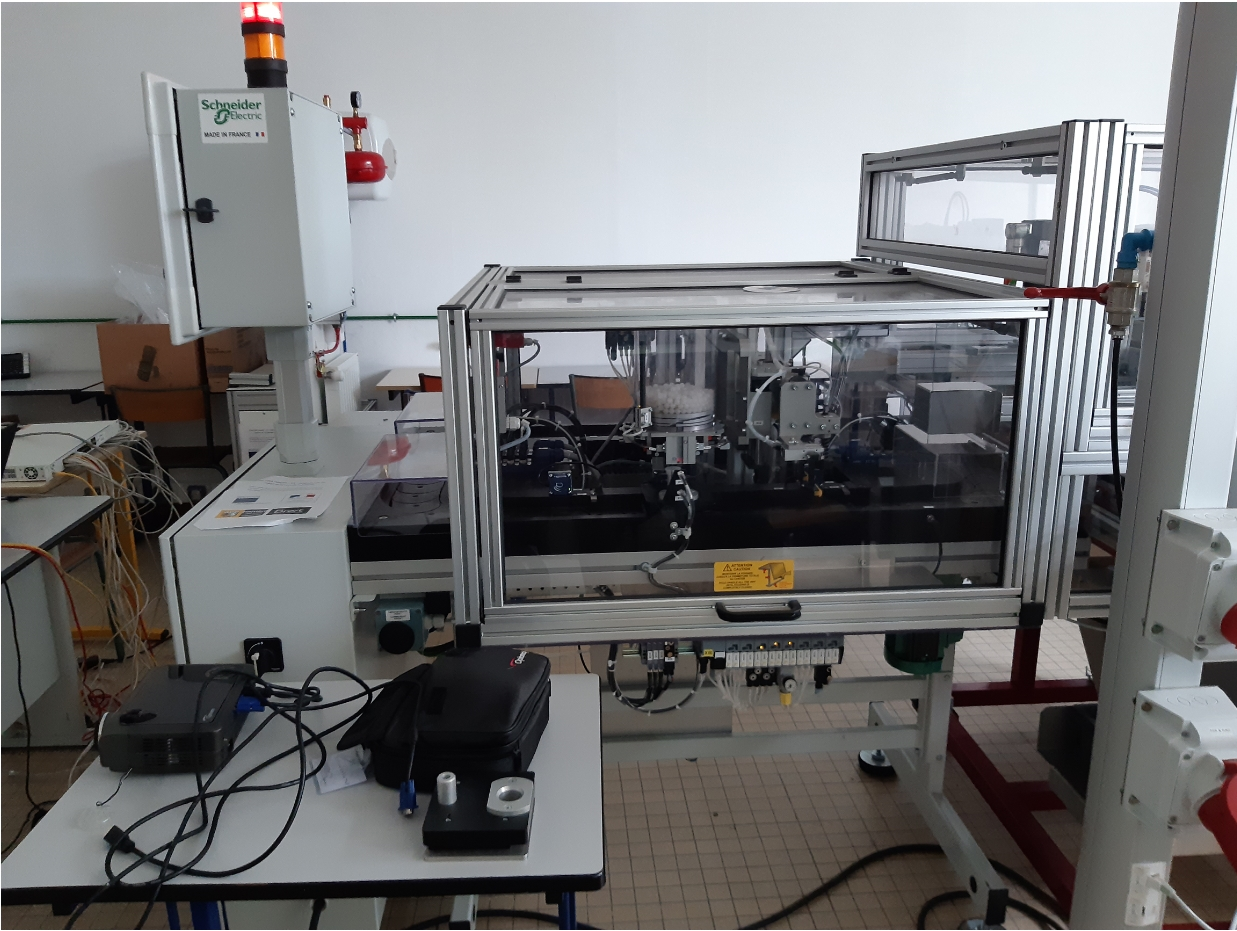
\includegraphics[scale=0.28]{plateforme.jpg}
			\label{fig:plateforme}
		\end{figure}
	\end{frame}
	
	\begin{frame}[allowframebreaks]
	\frametitle{Prise en main}
		\begin{block}{Unity Pro XLS}
				\begin{itemize}
					\setbeamertemplate{itemize item}[square]
					\item Différents types de registres : \%I, \%M, \%MW, \%Q
					\item Différents types de données : Array, Int, Bool, EBOOL\footnote{\url{https://www.se.com/in/en/faqs/FA86461/}}
				\end{itemize}
		\end{block}
		
		\begin{figure}[H]
			\centering
			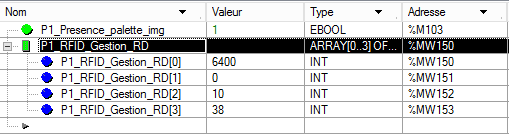
\includegraphics[scale=0.5]{unity.png}
			\label{fig:unity}
		\end{figure}
		
		\begin{figure}[H]
			\centering
			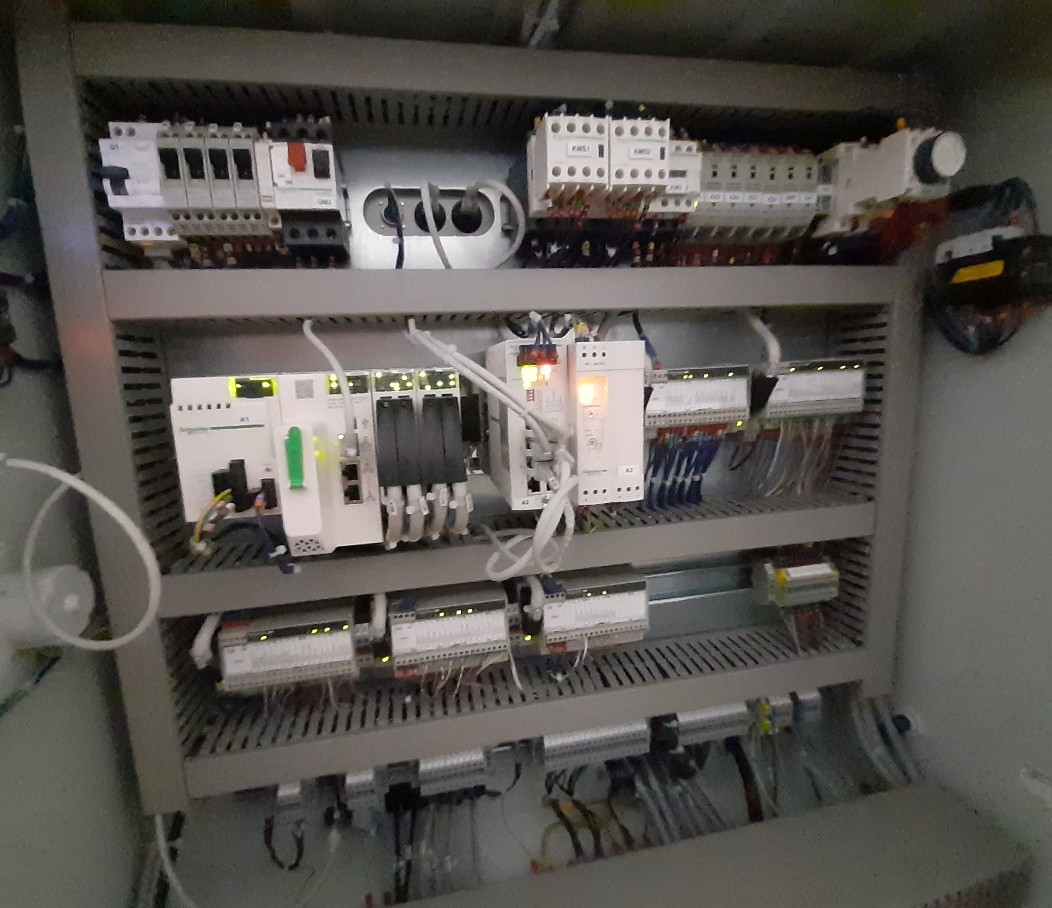
\includegraphics[scale=0.28]{automate.jpg}
			\label{fig:automate}
		\end{figure}
	\end{frame}
	
	% ---------------------------------------------------------------- %
	\subsection{Récupération des valeurs des registres}
	\begin{frame}[allowframebreaks]
	\frametitle{Programme Java}
		\begin{block}{Étapes}
				\begin{enumerate}
					\item Renseignements des valeurs (timer, nombre de répétitions de lecture, adresse, type, taille du registre à lire, ...)
					\item Connexion à la base de données
					\item Lecture des valeurs dans le registre demandé
					\item Affichage dans la console si disponible
					\item Enregistrement dans la base de données
				\end{enumerate}
		\end{block}
	\end{frame}
	
	\begin{frame}[allowframebreaks]
	\frametitle{Base de données}
		\begin{block}{MS SQL Server}
				\begin{itemize}
					\setbeamertemplate{itemize item}[square]
					\item Utilisation de MS SQL Server en localhost
					\item Obligation d'utiliser un driver SQL/Java
					\item Contenu :
						\begin{itemize}
							\setbeamertemplate{itemize item}[cercle]
							\item currDataTime $\rightarrow$ type 'dateTime', non NULL
							\item registerName $\rightarrow$ type nChar(15), NULL
							\item registerValue $\rightarrow$ type int, NULL
						\end{itemize}
				\end{itemize}
		\end{block}
		
		\begin{figure}[H]
			\centering
			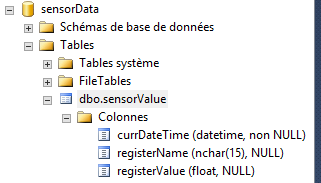
\includegraphics[scale=0.3]{dataBase.png}
			\label{fig:db}
		\end{figure}
	\end{frame}
	
	\subsubsection{Résultats}
	\begin{frame}[allowframebreaks]
	\frametitle{Résultats}
		\begin{figure}[H]
			\centering
			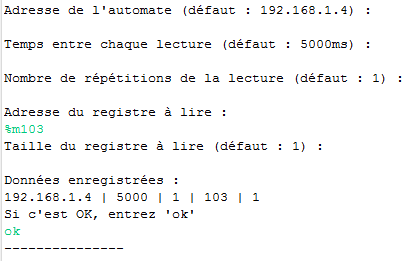
\includegraphics[scale=0.25]{test1.png}
			\label{fig:test1}
		\end{figure}
		
		\begin{figure}[H]
			\centering
			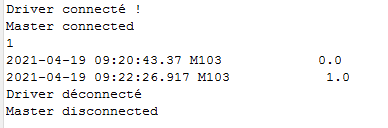
\includegraphics[scale=0.3]{test3.png}
			\label{fig:test3}
		\end{figure}
		
		\begin{figure}[H]
			\centering
			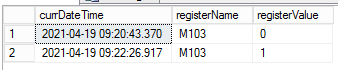
\includegraphics[scale=0.4]{dataBase2.png}
			\label{fig:db2}
		\end{figure}

		\begin{figure}[H]
			\centering
			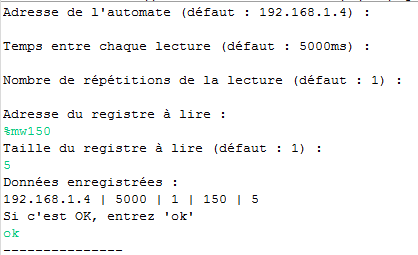
\includegraphics[scale=0.3]{test4.png}
			\label{fig:test4}
		\end{figure}
		
		\begin{figure}[H]
			\centering
			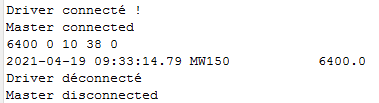
\includegraphics[scale=0.3]{test5.png}
			\label{fig:test5}
		\end{figure}
	\end{frame}
	
	% ---------------------------------------------------------------- %
	\subsection{Analyse des besoins matériels pour le drone}
	\begin{frame}[allowframebreaks]
	\frametitle{Drone}
		\begin{block}{Capteurs}
				\begin{itemize}
					\setbeamertemplate{itemize item}[square]
					\item Caméra
					\item Raspberry Pi
					\item Batterie pour le RPi
					\item Capteurs de distances
					\item Positionnement dans la pièce (survol de l'anomalie)
				\end{itemize}
		\end{block}
	\end{frame}
	
	% ---------------------------------------------------------------- %
	\section{A faire}
	\begin{frame}[allowframebreaks]
	\frametitle{A faire}
		\begin{alertblock}{}
				\begin{itemize}
					\setbeamertemplate{itemize item}[triangle]
					\item Connexion au drone via le port UART et Raspberry Pi
					\item Communication entre le drone et le Raspberry Pi
					\item Accès aux capteurs internes et intéraction avec le SDK du drone
				\end{itemize}
		\end{alertblock}
	\end{frame}
	
	% ---------------------------------------------------------------- %
	\section*{Remerciements}
	\begin{frame}
	\frametitle{Remerciements}
		\begin{center}
		Merci pour votre attention!

		\bigbreak
		Avez-vous des questions?
		\end{center}
	\end{frame}
	% ---------------------------------------------------------------- %
	
	%\section*{Bibliographie}
	%\begin{frame}[allowframebreaks]
	%\frametitle{Bibliographie}
		%\bibliographystyle{unsrt}
		%\bibliography{bibliographie}
	%\end{frame}
	% ---------------------------------------------------------------- %
\end{document}